\section{Designing API Endpoints}\label{sec:generalEP}
This section deals with completing the following:
\begin{center}
\userstory{As a developer, I want a design of the model for Sequence and a guideline for implementing this, such that I can concentrate on actually implementing the model.}
\medskip
\userstory{As a developer, I want a design of the model for WeekSchedule and a guideline for implementing this, such that I can concentrate on actually implementing the model.}
\end{center}

\noindent
First a presentation of the steps involved in developing the different layers for the REST API.
This is followed by the design of the model as a class diagram.

\subsection{Developing an Endpoint and its Constituents}\label{subsec:general}
As stated in \myref[name]{sec:architecture} a single endpoint consists of three layers.
A core layer which is where the classes of the model are implemented and tested.
A persistence layer which is where the tables for the model, defined in the core, are created; the annotations from hibernate used in the core relates the data in the two layers.
The persistence layer for each of the endpoints, also consists of a Data Access Object(DAO) class which is used to gain access to the objects in the database.
The last layer is the service layer which is what is called from any application using HTTP requests.

\subsubsection{The Core Layer}
The first layer to be implemented for an endpoint is the core layer.
Implementing this layer is done in two steps:
\begin{description}
	\item[Creating the classes needed for the endpoint] \hfill \\
	When creating the classes all fields of the classes are annotated with Hibernate annotations which in turn helps retrieve the correct objects when querying the database.
	The annotations can create relationship tables, which makes creating relationships between entities a simple task.
	What is important for this layer is to make sure that the correct annotations are used and making sure that the design has been thoroughly inspected in order to ensure it is sensible.
	The methods created on the classes should be methods which will be used in GIRAF applications on the object, like adding another pictogram to a week schedule.
	\item[Unit testing the classes] \hfill \\
	There must be unit tests which creates some objects of the class and use the methods implemented on them.
	There should be enough unit tests such that all non-simple methods like a simple add, or getters and setter have 100\% code coverage.
	We do not want to test methods which are simply adding an element to a Java list implementation, Java's methods are thoroughly tested and more tests are therefore unnecessary. 
\end{description}

\noindent
\subsubsection{The Persistence Layer}
The persistence layer consists of four steps

\begin{description}
	\item[Creating the Tables from the Core] \hfill \\
	The first task is to create the tables specified in the core layer as SQL.
	Any class annotated with \texttt{@Entity} and \texttt{@Table(name = "name")} needs to have a corresponding table created for them.
	If a class has a many-to-many relation with another class the SQL needs to create the relationship-table, or the join-table, you can also add extra properties on these join-tables as e.g. an index.
	As we are developing incrementally on the REST API any alterations to a class may require subsequent alterations to the related tables, this should also be done in this step.
	If we perform any alterations to a table the already existing data is migrated to fit in the new tables such that no information is lost.
	\item[Creating Data] \hfill \\
	The next step is to create example data for the new tables created in the step before such that we can create test for the DAOs to be created in the next step.
	\item[Creating a DAO for the endpoint] \hfill \\
	First an interface is created which must extend from \texttt{BaseDao}, this interface should contain the methods to be implemented for the DAO.
	The DAO consists of methods that query the database according to certain search criteria and are also named as such.
	Each DAO should only contain methods that will actually be used by the class they pertain to, e.g. GIRAF never has to find all week schedules containing a specific pictogram, therefore a \texttt{getAll(Frame pictogram)} should not exist.
	Similarly the DAO should also only contain methods to get objects which cannot already be retrieved by another DAO in the same manner,	e.g. \texttt{getByUser(User user)} may seem like a relevant method for \texttt{WeekScheduleDao}, but users already have a collection of all their week schedules so this method is never needed.

	Once all the necessary methods are added to the interface it is implemented in a class that inherits from a \texttt{BaseDaoImpl} class which implements the \texttt{BaseDao} Interface, which implements the basic operations of adding, removing and updating an element.
	\item[Testing the DAO] \hfill \\
	Lastly the DAO will have to be tested through integration tests on the data created in step 2 of this layer.
	The tests should be created such that we know whether all entities are retrieved correctly and also test whether wrong information is retrieved or not.
	The tests here are not only used to make sure the DAOs retrieve the correct information, but also to test whether the annotations in the core layer have been used correctly and that the design works as intended.
\end{description}

\subsubsection{The Service Layer}
The final layer to create for an endpoint is the service layer and consists of a single step:
\begin{description}
	\item[Creating HTTP Request Response Methods]\hfill \\
	Here we have to think about the context the endpoint will be used in and create methods for any requests that might occur in this context, these methods are annotated with JAX-RS annotations which RESTEasy will use, as mentioned in \myref{sec:techstack}.
	The methods will use the DAOs from the persistence layer to retrieve the requested data and send this data back as JSON which is serialised by Jackson which is also described in\myref{sec:techstack}.
	We do not have any automatic tests for this as they use methods which are already tested and because the Jackson library is heavily tested.
	Instead the way we test the service layer is to manually test whether the methods behaves in the intended way.
\end{description}
\noindent
The next section will present the model to be modelled in the core layer for the three endpoints, which we are developing during this sprint.

\subsection{The Updated Model for Objects in GIRAF}\label{subsec:model}
The new model design is an attempt to make the central parts of GIRAF more cohesive than before.
The class diagram can be seen on \myref{fig:fullmodelclassdiagram}, excessive detail have been removed.
We will start by discussing week schedule and then go on to discuss the rest of the model.

\begin{figure}[h]
    \centering
    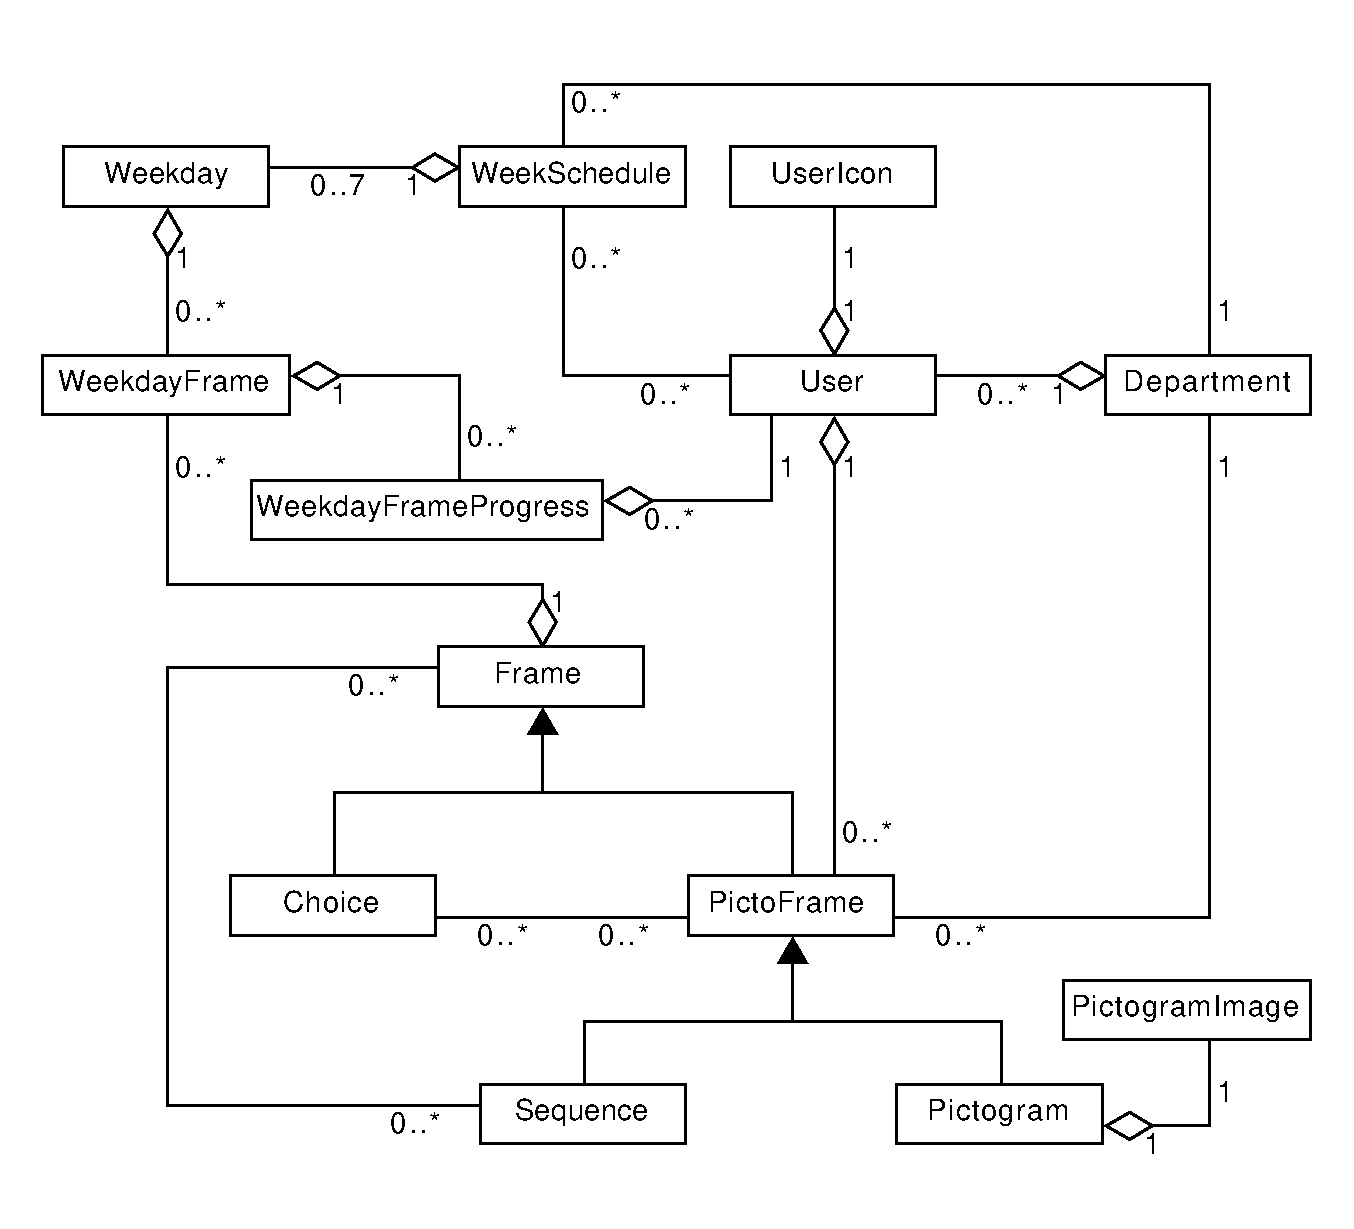
\includegraphics[width=0.75\textwidth]{figures/fullclassdiagram.pdf}
    \caption{Classdiagram of the new model used in the REST API}\label{fig:fullmodelclassdiagram}
\end{figure}

A week schedule consists of seven week days, one for each day of the week, which creates a relation from a \texttt{weekSchedule} to several \texttt{weekDay}s.
We acknowledge that a weekday is supposed to be able to use the following in its schedule: 
\begin{multicols}{3}
\begin{itemize}
	\item \texttt{Sequence}s
	\item \texttt{Pictogram}s
	\item \texttt{Choice}s
\end{itemize}     
\end{multicols}

With this in mind we created a super class which all these can inherit from, and from this we can make it so a week schedule for each day has a list of this super class, which we call \texttt{Frame}.
\myref{fig:fullmodelclassdiagram} shows how the only connection from these three elements of a weekday is through the \texttt{Frame} class.
We can also encapsulate common data in this super class.
We made a distinction between \texttt{Choice}s, \texttt{Sequence}s, and \texttt{Pictogram}s, because a \texttt{Choice} in GIRAF does not contain as much of this common information as \texttt{Pictogram}s and \texttt{Sequence}s like a title or an owner.
Therefore \texttt{Sequence}s and \texttt{Pictogram}s inherit from yet another superclass called \texttt{PictoFrame}, that inherits from \texttt{Frame}, which encapsulate the common data between \texttt{Sequence}s and \texttt{Pictogram}s.
This also solves the problem of directly nested choices because a \texttt{Choice} can then have one--to--many of these \texttt{PictoFrame}s.
A \texttt{Sequence} has an ordered one--to--many relation to \texttt{Frame} and a \texttt{Pictogram} has a \texttt{PictogramImage} that separates a \texttt{Pictogram} from its associated image.
All these classes are very intertwined and rely on each other which makes the implementation somewhat difficult to work on in parallel in the group.
A \texttt{WeekSchedule} is owned by one or many \texttt{User}s, and it also belongs to a single department which the users also belong to.
All \texttt{PictoFrame}s are owned by a \texttt{User} and/or a \texttt{Department}.
There exists 3 kinds of users in the REST API, User which is the base level that all other users have, this includes citizens; Guardians which is used for the guardians at the institutions, and SuperUser which is an administration level user, that can administrate public pictograms.

The \texttt{weekday} has a relationship--class: \texttt{weekdayFrame} to bind these \texttt{Frame}s together with a weekday which preserves the order of frames on a weekday as well as being able to save the progress of a week schedule.
The progress is saved in another relationship--class: \texttt{weekdayFrameProgress} as the progress depends on the user because this new model of GIRAF week schedules allows a week schedule to be shared between users, which might be used for when an institution goes on a trip.

With the model described the following sections goes into more detail about the specific endpoints.
